\documentclass[letterpaper,addpoints,answers]{exam}
\usepackage{graphicx}
\usepackage{multicol}
\usepackage{wrapfig}
\usepackage{tikz}

\usetikzlibrary{calc}

\makeatletter
\def\grd@save@target#1{%
  \def\grd@target{#1}}
\def\grd@save@start#1{%
  \def\grd@start{#1}}
\tikzset{
  grid with coordinates/.style={
    to path={%
      \pgfextra{%
        \edef\grd@@target{(\tikztotarget)}%
        \tikz@scan@one@point\grd@save@target\grd@@target\relax
        \edef\grd@@start{(\tikztostart)}%
        \tikz@scan@one@point\grd@save@start\grd@@start\relax
        \draw[minor help lines] (\tikztostart) grid (\tikztotarget);
        \draw[major help lines] (\tikztostart) grid (\tikztotarget);
        \grd@start
        \pgfmathsetmacro{\grd@xa}{\the\pgf@x/1cm}
        \pgfmathsetmacro{\grd@ya}{\the\pgf@y/1cm}
        \grd@target
        \pgfmathsetmacro{\grd@xb}{\the\pgf@x/1cm}
        \pgfmathsetmacro{\grd@yb}{\the\pgf@y/1cm}
        \pgfmathsetmacro{\grd@xc}{\grd@xa + \pgfkeysvalueof{/tikz/grid with coordinates/major step x}}
        \pgfmathsetmacro{\grd@yc}{\grd@ya + \pgfkeysvalueof{/tikz/grid with coordinates/major step y}}
        \foreach \x in {\grd@xa,\grd@xc,...,\grd@xb}
        \node[anchor=north] at (\x,\grd@ya) {\pgfmathprintnumber{\x}};
        \foreach \y in {\grd@ya,\grd@yc,...,\grd@yb}
        \node[anchor=east] at (\grd@xa,\y) {\pgfmathprintnumber{\y}};
      }
    }
  },
  minor help lines/.style={
    help lines,
    gray,
    line cap =round,
    xstep=\pgfkeysvalueof{/tikz/grid with coordinates/minor step x},
    ystep=\pgfkeysvalueof{/tikz/grid with coordinates/minor step y}
  },
  major help lines/.style={
    help lines,
    line cap =round,
    line width=\pgfkeysvalueof{/tikz/grid with coordinates/major line width},
    xstep=\pgfkeysvalueof{/tikz/grid with coordinates/major step x},
    ystep=\pgfkeysvalueof{/tikz/grid with coordinates/major step y}
  },
  grid with coordinates/.cd,
  minor step x/.initial=.5,
  minor step y/.initial=.2,
  major step x/.initial=1,
  major step y/.initial=1,
  major line width/.initial=1pt,
}
\makeatother

\tikzset{
    right angle quadrant/.code={
        \pgfmathsetmacro\quadranta{{1,1,-1,-1}[#1-1]}     % Arrays for selecting quadrant
        \pgfmathsetmacro\quadrantb{{1,-1,-1,1}[#1-1]}},
    right angle quadrant=1, % Make sure it is set, even if not called explicitly
    right angle length/.code={\def\rightanglelength{#1}},   % Length of symbol
    right angle length=2ex, % Make sure it is set...
    right angle symbol/.style n args={3}{
        insert path={
            let \p0 = ($(#1)!(#3)!(#2)$) in     % Intersection
                let \p1 = ($(\p0)!\quadranta*\rightanglelength!(#3)$), % Point on base line
                \p2 = ($(\p0)!\quadrantb*\rightanglelength!(#2)$) in % Point on perpendicular line
                let \p3 = ($(\p1)+(\p2)-(\p0)$) in  % Corner point of symbol
            (\p1) -- (\p3) -- (\p2)
        }
    }
}

\begin{document}

\begin{coverpages}
 \large\bfseries
 
 \noindent 
 Physics 107: Physics for Life-Sciences

 \vspace{2ex}
 \noindent
 Midterm Exam: November 16, 2015

 \vspace{3ex}
 \noindent 
 This test is administered under the rules and regulations of the honor code of the College of William \& Mary.

 \vspace{2ex}
 \noindent 
 Name:\enspace\makebox[2.3in]{\hrulefill} \\

 \noindent 
 Signature:\enspace\makebox[2in]{\hrulefill} \\

 \vspace{5ex}
 \noindent 
 Instructions:
 \begin{itemize}
  \item This is a closed book, closed notes test.
  \item Calculators are NOT needed and NOT allowed. Devices with wireless connections are NOT allowed.
  \item Start your work from the fundamental equations on the formula sheet, and derive any additional expressions that you may need.
  \item Circle your answer for each part of each problem. 
  \item Clearly mark out any work that you wish the grader to disregard.  Do not waste your time erasing.
  \item Your work will be graded based on your ability to write down a logical and organized solution grounded in the correct assessment of the physics of a situation. No credit will be given for an answer that is not justified by a logical solution or where that justification is not organized or readable. Partial credit will be given up to the point where your solution departs from a correct analysis of the physics involved for any given part of a problem.
 \end{itemize}

 \pagebreak

 \begin{center}
  \gradetable[v][questions]
 \end{center}
 
\end{coverpages}
 

\begin{questions}

\printanswers

% 3 multiple choice questions

\begin{question}[5]
\begin{multicols}{2}
A container, closed on the right side but open to atmosphere on the left side, is almost completely filled with water as shown on the figure. Three points in the container are marked on the figure. Rank the points according to their pressures, from highest to lowest.
\begin{checkboxes}
 \correctchoice $P_A = P_B > P_C$
 \choice $P_B > P_A > P_C$
 \choice $P_B > P_A = P_C$
 \choice $P_C > P_B > P_A$
 \choice $P_C > P_A = P_B$
\end{checkboxes}
\begin{center}
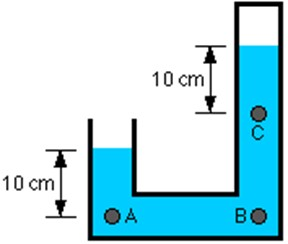
\includegraphics[width=0.3\textwidth]{test3/container_pressure}
\end{center}
\end{multicols}
\end{question}

\begin{question}[5]
A wooden block with a weight of 100\,N floats exactly 50\% submerged in a liquid. The upward buoyant force exerted on the block by the liquid\ldots
\begin{checkboxes}
 \choice is exactly 50\,N.
 \correctchoice is exactly 100\,N.
 \choice depends on the density of the block.
 \choice depends on the density of the liquid.
 \choice depends on both the density of the block and the liquid.
\end{checkboxes}
\end{question}

\begin{question}
\begin{multicols}{2}
You have an axe to grind. The grindstone has a mass $M$ of 90\,kg, a radius $R$ of $\frac{1}{3}$\,m and is initially turning at 90\,rpm. It can be modeled as a disk with moment of inertia $I = \frac{1}{2} M R^2$.

You press the steel axe against the grindstone with a radial force of 30\,N. The coefficient of kinetic friction between steel and stone is $\mu_k = 0.2$.
\begin{center}
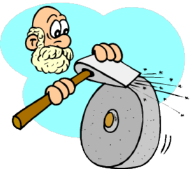
\includegraphics[width=0.2\textwidth]{test3/axe_to_grind}
\end{center}
\end{multicols}
\begin{parts}
\part[5] What is the torque on the grindstone?
\begin{checkboxes}
 \choice $1\,\mbox{N}\cdot\mbox{m}$
 \correctchoice $2\,\mbox{N}\cdot\mbox{m}$
 \choice $6\,\mbox{N}\cdot\mbox{m}$
 \choice $10\,\mbox{N}\cdot\mbox{m}$
 \choice $18\,\mbox{N}\cdot\mbox{m}$
\end{checkboxes}
\begin{solution}[1in]
If the radial force $N$ is 30\,N and the coefficient of friction $\mu_k = 0.2$, then the force of friction will be $f = 6$\,N. This means that the torque will be $\tau = f R = 6\,\mbox{N}\cdot \frac{1}{3}\,\mbox{m} = 2\,\mbox{N}\cdot\mbox{m}$.
\end{solution}
\part[5] What will be the angular acceleration as the stone grinds to a halt?
\begin{checkboxes}
 \choice 0.2\,rad/s$^2$
 \choice 0.5\,rad/s$^2$
 \choice 2.0\,rad/s$^2$
 \choice 3.0\,rad/s$^2$
 \correctchoice Another value, namely:\enspace\rule{2in}{0.4pt}\,rad/s$^2$
\end{checkboxes}
\begin{solution}
Together with a moment of inertia $I = \frac{1}{2} M R^2 = 5\,\mbox{kg}\cdot\mbox{m}^2$ the torque gives us $\alpha = \tau/I = f R/I = 2\,\mbox{N}\cdot\mbox{m}/5\,\mbox{kg}\cdot\mbox{m}^2 = 0.4\,\mbox{rad}/\mbox{s}^2.$
\end{solution}
\end{parts}
\end{question}

\pagebreak

\begin{question}
\begin{multicols}{2}
Even when the head is held erect, as in the figure below, its center of mass is not directly over the principal point of support (the atlanto-occipital joint). The muscles in the back of the neck must therefore exert a force to keep it erect. That is why your head falls forward when you fall asleep in class.

The perpendicular distance between the line of action for the weight of the head and the pivot point is $r_{W\perp} = 2.0$\,cm and the perpendicular distance between the line of action for the force the muscles exert on the head and the pivot point is $r_{M\perp} = 5.0$\,cm. Assume the weight of the head is $W = 50$\,N.
\begin{center}
 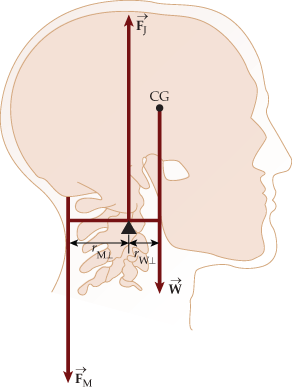
\includegraphics[width=0.26\textwidth]{test3/head}
\end{center}
\end{multicols}
\begin{parts}
 \part[5] What is the force exerted by the muscles?
 \begin{solution}[2in]
 The net torque around the point of support must be zero, or $\tau_{net} = r_{M\perp} F_M - r_{W\perp} W = 0$. This leads to $$F_M = \frac{r_{W\perp}}{r_{M\perp}} W = \frac{2.0\,\mbox{cm}}{5.0\,\mbox{cm}} 50\,\mbox{N} = 20\,\mbox{N}.$$
 \end{solution}
 \part[5] What is the force $F_J$ on the point of support?
 \begin{solution}[2in]
 The net force on the head must be zero, or $F_{net} = F_j - F_M - W = 0$. This leads to $$F_j = F_M + W = 20\,\mbox{N} + 50\,\mbox{N} = 70\,\mbox{N}.$$
 \end{solution}
\end{parts}
\end{question}

\pagebreak

\begin{question}
\begin{multicols}{2}
You place a beaker that is two-thirds full of water with a density of $\rho_{H_2O} = 1000$\,kg/m$^3$ on a laboratory scale. You then use a light-weight cord to suspend an aluminum object with density $\rho_{Al} = 2700$\,kg/m$^3$ in the water. The object is completely submerged, and none of the water spills out of the beaker. You observe that the reading on the scale increases by $\Delta m = 0.0027$\,kg. You may approximate the magnitude of the gravitational acceleration $g$ as $10.0\,\mbox{m}/\mbox{s}^2$.
\begin{center}
 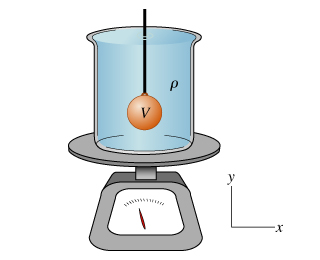
\includegraphics[width=0.3\textwidth]{test3/beaker}
\end{center}
\end{multicols}
\begin{parts}
 \part[5] In words, what is the reason the scale reads a larger weight?
 \begin{solution}[1in]
 The force of buoyancy pushes the aluminum object upwards, but Newton's 3rd law requires that the object will push down on the water (and the scale) with the same magnitude.
 \end{solution}
 \part[10] What is the volume of the object?
 \begin{solution}[2in]
 Because the buoyant force $F_B$ is equal to the weight of the displace liquid $\rho_{H_2O} V g$, this will also be the additional force on the scale. That will result in an additional reading $\Delta m = \rho_{H_2O} V$. The volume is therefore $$V = \frac{\Delta m}{\rho_{H_2O}} = \frac{0.0027\,\mbox{kg}}{1000\,\mbox{kg}/\mbox{m}^3} = 2.7 \times 10^{-6}\,\mbox{m}^3 = 2.7\,\mbox{cm}^3.$$
 \end{solution}
 \part[5] How much does the tension in the cord change when the object is submerged?
 \begin{solution}[1in]
 The tension decreases by the buoyant force, $\rho_{H_2O} V g = \Delta m g = 0.027\,\mbox{N}$.
 \end{solution}
\end{parts}
\end{question}

\pagebreak

\begin{question}
A 10\,m-long horizontal garden hose with a diameter 0.016\,m has at the end a nozzle with a diameter 0.008\,m. Water flows through the hose at a velocity of $v_h = 2$\,m/s. Assume for parts a and b that the water has no viscosity or other form of energy dissipation, and that the density of water is 1000\,kg/m$^3$.
\begin{parts}
 \part[5] What is the velocity of the water as it comes out of the nozzle?
 \begin{solution}[1.5in]
 Using the continuity equation we can determine the velocity in the hose: $A_h v_h = A_n v_n$. This gives use $$v_n = \frac{A_h}{A_n} v_h = \frac{r_h^2}{r_n^2} v_h = \left( \frac{r_h}{r_n} \right)^2 v_h = 2^2 \cdot 2\,\mbox{m}/\mbox{s} = 4 \cdot 8\,\mbox{m}/\mbox{s} = 8\,\mbox{m}/\mbox{s}.$$
 \end{solution}
 \part[5] What is the pressure difference between the water in the hose and water in the nozzle?
 \begin{solution}[2.5in]
 Using Bernoulli's equation we can determine the difference between $P_h$ and $P_n$: $$P_h - P_n = \frac{1}{2} \rho v_n^2 - \frac{1}{2} \rho v_h^2 = \frac{1}{2} \rho (v_n^2 - v_h^2) = \frac{1}{2} 1000\,\mbox{kg}/\mbox{m}^3 (64 - 4) (\mbox{m}/\mbox{s})^2 = 30 \cdot 10^3\,\mbox{Pa}.$$
 \end{solution}
 \part[10] The viscosity of the water ($\eta = 10^{-3}\,\mbox{Pa}\cdot\mbox{s}$) will cause a pressure drop $\Delta P$ as the water flows through the garden hose. What will be the magnitude of this pressure drop? How does this compare to your answer in part b? \emph{Hint:} Allow factors of $\pi$ to drop out in the algebra before starting your numerical calculations.
 \begin{solution}[2in]
 Using Poisseuille's law we can relate the pressure drop $\Delta P$ to the given parameters of the garden hose: $$\Delta P = \frac{8 \eta \ell Q}{\pi r_h^4} = \frac{8 \eta \ell A_h v_h}{\pi r_h^4} = \frac{8 \eta \ell \pi r_h^2 v_h}{\pi r_h^4} = \frac{8 \eta \ell v_h}{r_h^2} = \frac{8 \cdot 10^{-3}\,\mbox{Pa}\cdot\mbox{s} \cdot 10\,\mbox{m} \cdot 2\,\mbox{m}/\mbox{s}}{(8\cdot 10^{-3}\,\mbox{m})^2} = 2.5 \cdot 10^3\,\mbox{Pa}$$.
 \end{solution}
\end{parts}
\end{question}

\end{questions}

 \pagebreak
 
 {\Large Possibly useful relations (feel free to detach this page):}
  
% Test 1
%  \fontseries{\seriesdefault}
%  \begin{multicols}{2}
%  \Large
%  \noindent
%  $\vec{v}_{avg} = \Delta\vec{x} / \Delta t$ \\
%  $x = x_0 + v_0 t + \frac{1}{2} a t^2$ \\
%  $v^2 = v_0^2 + 2 a (x - x_0)$ \\
%  $R = \frac{v_0^2}{g}\sin 2\theta$ \\
%  $\vec{F}_{net} = m \vec{a}$ \\
%  $\vec{W} = m \vec{g}$ \\
%  $\cos\theta = \hbox{adjacent}/\hbox{hypotenuse}$ \\
%  $\sin\theta = \hbox{opposite}/\hbox{hypotenuse}$ \\
%  $\sin 30^\circ = \cos 60^\circ = \frac{1}{2}$ \\
%  $\cos 30^\circ = \sin 60^\circ = \frac{\sqrt{3}}{2}$ \\
 
%  \noindent
%  $\vec{a}_{avg} = \Delta\vec{v} / \Delta t$ \\
%  $v = v_0 + a t$ \\
%  $v_{avg} = \frac{v_0 + v}{2}$ \\
%  $h = \frac{v_0^2}{2 g} \sin^2 \theta$ \\
%  $\vec{F}_{BA} = - \vec{F}_{AB}$ \\
%  $\vec{g} = 9.80\,m/s^2$ downward \\
%  $x = \frac{-b \pm \sqrt{b^2 - 4 a c}}{2 a}$ \\
%  $\tan\theta = \sin\theta / \cos\theta$ \\
%  $\tan 45^\circ = 1$ \\
%  \end{multicols}


% Test 2
%  \fontseries{\seriesdefault}
%  \begin{multicols}{2}
%  \Large
%  \noindent
%  $\vec{v}_{avg} = \Delta\vec{x} / \Delta t$ \\
%  $\vec{a}_{avg} = \Delta\vec{v} / \Delta t$ \\
%  $x = x_0 + v_0 t + \frac{1}{2} a t^2$ \\
%  $v = v_0 + a t$ \\
%  $v_{avg} = \frac{v_0 + v}{2}$ \\
%  $v^2 = v_0^2 + 2 a (x - x_0)$ \\
%  $\vec{F}_{net} = m \vec{a}$ \\
%  $\vec{F}_{BA} = - \vec{F}_{AB}$ \\
%  $W = F d \cos\theta$ \\
%  $W_{net} = -\Delta PE = \Delta KE$ \\
%  $KE = \frac{1}{2} m v^2$ \\
%  $PE_k = \frac{1}{2} k x^2$ \\
%  $PE_g = m g h$ \\
%  $KE_i + PE_i + W_{nc} = KE_f + PE_f$ \\
%  $P = \frac{W}{\Delta t}$ \\
%  $\hbox{Eff} = \frac{W_{out}}{E_{in}}$ \\
%  $\cos\theta = \hbox{adjacent}/\hbox{hypotenuse}$ \\
%  $\sin\theta = \hbox{opposite}/\hbox{hypotenuse}$ \\
%  $\tan\theta = \sin\theta / \cos\theta$ \\
%  $\sin 30^\circ = \cos 60^\circ = \frac{1}{2}$ \\
%  $\cos 30^\circ = \sin 60^\circ = \frac{\sqrt{3}}{2}$ \\
%  $\tan 45^\circ = 1$ \\

%  \noindent
%  $R = \frac{v_0^2}{g}\sin 2\theta$ \\
%  $h = \frac{v_0^2}{2 g} \sin^2 \theta$ \\
%  $0 \le f_s \le \mu_s N$ \\
%  $f_k = \mu_k N$ \\
%  $\frac{F}{A} = Y \frac{\Delta L}{L}$ \\
%  $F_k = -k x$ \\
%  $\vec{W} = m \vec{g}$ \\
%  $\vec{g} = 9.80\,\mbox{m}/\mbox{s}^2$ downward \\
%  $F_G = G \frac{m M}{r^2}$ \\
%  $G = 6.67 \times 10^{-11}\,\mbox{N}\cdot\mbox{m}^2/\mbox{kg}^2$ \\
%  $\vec{I} = \vec{F}_{avg} \Delta t$ \\
%  $\vec{p} = m \vec{v}$ \\
%  $\vec{F}_{net} = \frac{\Delta \vec{p}}{\Delta t}$ \\
%  $v_1 - v_2 = v'_2 - v'_1$ \\
%  $\theta = \frac{s}{r}$ \\
%  $v = r \omega$ \\
%  $f = \frac{1}{T}$ and $\omega = 2 \pi f = \frac{2 \pi}{T}$ \\
%  $a_c = \frac{v^2}{r} = r \omega^2$ \\
%  $F_c = m\frac{v^2}{r} = m r \omega^2$ \\
%  $1\,\hbox{cal} = 4.186$\,J and $1\,\hbox{Cal} = 1000$\,cal \\ 
%  $x = \frac{-b \pm \sqrt{b^2 - 4 a c}}{2 a}$ \\
%  \end{multicols}


% Test 3
 \fontseries{\seriesdefault}
 \begin{multicols}{2}
 \large
 \noindent
 $\vec{v}_{avg} = \Delta\vec{x} / \Delta t$ \\
 $\vec{a}_{avg} = \Delta\vec{v} / \Delta t$ \\
 $x = x_0 + v_0 t + \frac{1}{2} a t^2$ \\
 $v = v_0 + a t$ \\
 $v_{avg} = \frac{v_0 + v}{2}$ \\
 $v^2 = v_0^2 + 2 a (x - x_0)$ \\
 $\vec{F}_{net} = m \vec{a}$ \\
 $\vec{F}_{BA} = - \vec{F}_{AB}$ \\
 $W = F d \cos\theta$ \\
 $W_{net} = -\Delta PE = \Delta KE$ \\
 $P = \frac{W}{\Delta t}$ \\
 $\hbox{Eff} = \frac{W_{out}}{E_{in}}$ \\
 $KE_i + PE_i + W_{nc} = KE_f + PE_f$ \\
 $PE_k = \frac{1}{2} k x^2$ \\
 $PE_g = m g h$ \\
 $KE_{trans} = \frac{1}{2} m v^2$ \\
 $KE_{rot} = \frac{1}{2} I \omega^2$ \\
 $I_{point} = M R^2$ \\
 $I_{disk} = \frac{1}{2} M R^2$ \\
 $I_{sphere} = \frac{2}{5} M R^2$ \\
 $P = \frac{F}{A}$ \\
 $P_{gauge} = P - P_{atm}$ \\
 $\rho = \frac{M}{V}$ \\
 $\rho_{water} = 10^3\,\hbox{kg}/\hbox{m}^3$ \\
 $Q = \frac{\Delta V}{\Delta t} = A v$ \\
 $Q = \frac{\Delta P \pi r^4}{8 \eta L}$ \\
 $\hbox{Power} = P Q$ \\
 $A \cdot v = \hbox{constant}$ \\
 $P + \rho g y + \frac{1}{2} \rho v^2 = \hbox{constant}$ \\
 $F_B = \rho g V_{displaced}$ \\
 $F_{ST} = \gamma L$ \\
 $P = \frac{4 \gamma}{r}$ \\
 $h = \frac{2 \gamma \cos\theta}{\rho g r}$ \\
 $N_R = \frac{\rho v L}{\eta} = \frac{2 \rho v r}{\eta}$ \\
 $x = \frac{-b \pm \sqrt{b^2 - 4 a c}}{2 a}$ \\

 \noindent
 $R = \frac{v_0^2}{g}\sin 2\theta$ \\
 $h = \frac{v_0^2}{2 g} \sin^2 \theta$ \\
 $0 \le f_s \le \mu_s N$ \\
 $f_k = \mu_k N$ \\
 $\frac{F}{A} = Y \frac{\Delta L}{L}$ \\
 $F_k = -k x$ \\
 $\vec{W} = m \vec{g}$ \\
 $\vec{g} = 9.80\,\mbox{m}/\mbox{s}^2$ downward \\
 $F_G = G \frac{m M}{r^2}$ \\
 $G = 6.67 \times 10^{-11}\,\mbox{N}\cdot\mbox{m}^2/\mbox{kg}^2$ \\
 $\vec{I} = \vec{F}_{avg} \Delta t$ \\
 $\vec{p} = m \vec{v}$ \\
 $\vec{F}_{net} = \frac{\Delta \vec{p}}{\Delta t}$ \\
 $v_1 - v_2 = v'_2 - v'_1$ \\
 $\theta = \frac{s}{r}$ \\
 $v = r \omega$ \\
 $f = \frac{1}{T}$ and $\omega = 2 \pi f = \frac{2 \pi}{T}$ \\
 $a_c = \frac{v^2}{r} = r \omega^2$ \\
 $F_c = m\frac{v^2}{r} = m r \omega^2$ \\
 $\tau = r F \sin\theta = r_\perp F$ \\
 $\omega = \frac{\Delta \theta}{\Delta t}$ \\
 $\alpha = \frac{\Delta \omega}{\Delta t}$ \\
 $\tau = I \alpha$ \\
 $L = I \omega$ \\
 $\tau = \frac{\Delta L}{\Delta t}$ \\
 $x_{rms} = \sqrt{2 D t}$ \\
 $1\,\hbox{atm} = 10^5\,\hbox{Pa} = 760\,\hbox{mm}\cdot\hbox{Hg}$ \\
 $1\,\hbox{cal} = 4.186$\,J and $1\,\hbox{Cal} = 1000$\,cal \\ 
 $\cos\theta = \hbox{adjacent}/\hbox{hypotenuse}$ \\
 $\sin\theta = \hbox{opposite}/\hbox{hypotenuse}$ \\
 $\tan\theta = \sin\theta / \cos\theta$ \\
 $\sin 30^\circ = \cos 60^\circ = \frac{1}{2}$ \\
 $\cos 30^\circ = \sin 60^\circ = \frac{\sqrt{3}}{2}$ \\
 $\tan 45^\circ = 1$ \\
 \end{multicols}

\end{document}
